\documentclass[conference,compsoc]{IEEEtran}
\usepackage[pdftex]{graphicx}
\ifCLASSOPTIONcompsoc
  % IEEE Computer Society needs nocompress option
  % requires cite.sty v4.0 or later (November 2003)
  \usepackage[nocompress]{cite}
\else
  % normal IEEE
  \usepackage{cite}
\fi
\ifCLASSINFOpdf
  % declare the path(s) where your graphic files are
  % \graphicspath{{../pdf/}{../jpeg/}}
  % and their extensions so you won't have to specify these with
  % every instance of \includegraphics
  % \DeclareGraphicsExtensions{.pdf,.jpeg,.png}
\else
  % or other class option (dvipsone, dvipdf, if not using dvips). graphicx
  % will default to the driver specified in the system graphics.cfg if no
  % driver is specified.
  % \usepackage[dvips]{graphicx}
  % declare the path(s) where your graphic files are
  % \graphicspath{{../eps/}}
  % and their extensions so you won't have to specify these with
  % every instance of \includegraphics
  % \DeclareGraphicsExtensions{.eps}
\fi
\hyphenation{op-tical net-works semi-conduc-tor}

\begin{document}
\title{Procedural Maze-generation}
\author{\IEEEauthorblockN{Sigurt Bladt Dinesen}
\IEEEauthorblockA{IT University of Copenhagen\\
sidi@itu.dk}
}
\maketitle
\IEEEpeerreviewmaketitle
\section{Introduction}
%1. Introduction and problem statement
%What problem are you trying to solve? Why is this important?

Procedurally generation of levels that are well designed and don't break immersion is a common problem in game development. This is especially true for roguelikes which heavily rely on procedural content to keep the player engaged \cite{6Procedu79:online, BerlinIn39:online}. The specific approach varies from game to game, and only a few algorithms are simple and generic enough to be reused across projects.

This paper will introduce an algorithm that takes concepts from several other algorithms and puts it together in a new way. Specifically, the algorithm behaves like graph-grammars, but are applied to a lattice, so they some of the spatial properties of L-systems or cellular automata. We will therefore call this method Lattice-grammars.

We will go through what the algorithm is based on and how it works, before defining some test cases and evaluating the results.


\section{Background}
Has this been done before? How? If not, what's the closest related research?
(Both using similar approaches and other algorithms.) What's novel with your
research?

\subsection{L-Systems}

\subsection{Cellular Automata}

\subsection{Graph Grammars}

\subsection{Spelunky}


\section{(Game) Mechanics}
How does the game work that you are using? Why do you need AI in this game?

\subsection{Cops and Robbers}

Examples:
Pacman, horror games

Cop-win, some cul-de-sacs, low pitfalls, high cycle length?


\subsection{Dungeon Crawlers}

Examples:
Zelda, Binding of Issac

Choke-points?, cul-de-sacs, few cycles


\subsection{Theme}

Symmetry? Visual things?


\section{Methods}
First some definitions:
By \textit{lattice}, we mean a graph whose nodes are superimposed on a
(potentially infinite) square grid. More precisely, a lattice is a graph whose
nodes are coordinates in 2 dimensional Cartesian space, limited to $\{(x,y) \in
\mathbb{Z} \times \mathbb{Z}\}$, and which may have edges only between nodes
whose euclidean distance is exactly 1.

By \textit{maze} we mean a space of contiguous positions (discrete or not) that 
can be subdivided by walls in any fashion.

The overall method we use for generating mazes can be described as follows:

\begin{enumerate}
	\item We first discover (hopefully) interesting
		grammars, using an evolutionary algorithm.
	\item We create lattices from grammars, each describing the overall
		layout of a maze
	\item We create mazes from lattices. Each node in the lattice
		corresponding to a fixed-size room in the maze, connected to
		other blocks as described by the lattice.
\end{enumerate}

The three steps each involve numerous choices that can be tweaked in accordance
with with the type of maze one wishes to obtain.


\subsection{Lattice grammars}
A lattice grammar consists of a set of rules, where a rule is defined by a left-
and a right-hand lattice $(r_p, r_r)$. When a rule $(r_p,r_r)$ is applied to a
lattice, $r_p$ is used as a search pattern in the lattice.
If a match is found, the matching part of the lattice is transformed 
into $r_r$. The lattice is transformed by adding edges that are in $r_r$ but
not in $r_p$, and removing edges that are in $r_p$ but not in $r_r$.

An example of a grammar rule is shown in figure \ref{fig:simplerule}, and an
example of applying that rule to a lattice is shown in figure
\ref{fig:simplerule-applied}. In figure \ref{fig:simplerule-applied}, the rule
has been rotated 90-degrees counter-clockwise to find the match, and the lattice
is transformed accordingly to that rotation. Note that this is not the only
match in the lattice. A different, perhaps more obvious, match exists without
rotation.

\begin{figure}[hbp]
	\centering
	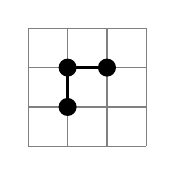
\begin{tikzpicture}
	%grid
	\draw [black!50,step=0.5] (0, 0) grid (1.5, 1.5);

	%nodes
	\foreach \p in {
		(0.5, 0.5),
		(0.5, 1),
		(1.0, 1)
	}\draw [thick, fill=black] \p circle (0.1);

	%paths
	\draw [very thick, color=black] plot coordinates {
		(0.5, 0.5)
		(0.5, 1)
		(1.0, 1)
	};

\end{tikzpicture}
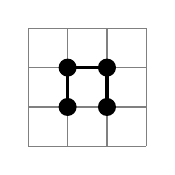
\begin{tikzpicture}
	%grid
	\draw [black!50,step=0.5] (0, 0) grid (1.5, 1.5);

	%nodes
	\foreach \p in {
		(0.5, 0.5),
		(0.5, 1),
		(1.0, 1),
		(1.0, 0.5)
	}\draw [thick, fill=black] \p circle (0.1);

	%paths
	\draw [very thick, color=black] plot coordinates {
		(0.5, 0.5)
		(0.5, 1)
		(1.0, 1)
		(1.0, 0.5)
	};

\end{tikzpicture}

	\caption{The left- and right-hand sides $(r_p,r_r)$ of a lattice-grammar rule that
	adds an edge}
	\label{fig:simplerule}
\end{figure}

\begin{figure}[hbp]
	\centering
	\input{graph-apply-plot.tex}
	\caption{A lattice that is matched by the rule in figure
	\ref{fig:simplerule} (left), and one possible result of applying the
	rule to the lattice (right)}
	\label{fig:simplerule-applied}
\end{figure}

The matching of a rule on a lattice might be implemented without rotation.
Without rotation in the matching process, the choice is deferred to the grammar,
which may or may not include different rotations of a rule. Intuitively,
including rotation in the matching process makes grammars less expressive, but
may help cause self-similarities in the resulting lattice. In practice, the
effect is not entirely obvious, and is tied to the method used to discover
grammars.

Another problem is how a grammar is applied. That is, in
addition to how a single rule is applied, there is the question of how the set
of rules that constitute a grammar is applied. If rules are applied in
succession, the order is significant, as one rule may alter the lattice in a way
that changes how the next rule applies. Of course, this is only true if
application may be done in-place, updating the lattice immediately with each
application. Alternatively, rules could be matched, and then applied together in
a single step. Furthermore, rules may be applied once, or once for each match.
Yet another approach could be to apply each rule repeatedly, continuing to the
next rule only when the first can't be matched to it's own result anymore.

\subsection{Maze generation}
The lattice describes the overall layout of the maze, but by considering the
lattice's nodes as fixed-size rooms, we can decouple the details of the maze layout
from the overall structure. Depending on the room-size, this stage can have
a profound impact on the final result. The connectivity of the maze can be
altered here, and the depth of cul-de-sacs can be decided. This stage has a
large visual impact as well. For example; for large room sizes, cul-de-sacs can
be difficult to discern visually on the lattice
level, and may be noticed only at the room level.


\subsection{Evolutionary algorithm}

We're using a very basic evolutionary algorithm to develop lattice-grammars that will generate environments that fit certain criteria. The overall algorithm looks like this:
\begin{itemize}
\item An initial population is created.
\item Until an termination criteria is met:
\begin{itemize}
    \item Randomly mutate the population
    \item Evaluate the population
    \item Select the best from the population to be parents for the next generation
    \item Breed the parents to create a new population
\end{itemize}
\end{itemize}

Each individual in a population is a list of rules that can be applied. They start out as empty rules that replaces nothing with nothing. The mutations that can be performed will then add or remove edges from the rules, or add another empty rule to the list. This is the genotype that will generate a lattice graph, the genotype.

To evaluate the population we use a mix of different metrics in a fitness function. Novelty search would also be a viable option, but was outside the scope of the project. The different metrics are weighted depending on which features of the graph should have the most influence.

For the selection process, the top 50\% ranking of the population is picked. This is one of the most basic elitist selection methods, but it's enough for us to achieve decent results, by simply discarding the individuals that did not mutate in a beneficial fashion.

For the final breeding step, we simplified the algorithm to simply pick randomly from parents and copy them. An actual breeding algorithm might improve the results, but because we got good results without, we determined that it was outside the scope of this project. If we were to extend the algorithm with actual breeding, we would take inspiration from the NEAT algorithm\cite{stanley:ec02}, to get proper crossover when combining graphs.

The evolution algorithm terminates after a certain number of generations, after which the best five mazes will be shown.


\subsection{Experiments}
In order to meet the criteria described in section \ref{sec:mechanics}, we run
several evolutionary experiments, with different fitness criteria.

\subsubsection{Cops and Robbers}
For games in the Cops and Robbers category, we try to evolve grammars that have
few but some pitfalls, few cul-de-sacs and a small average travel distance
between nodes. This should favour high-connectivity mazes with a few dead-ends,
providing "don't think just run" levels, sprinkled with a few traps created by
cul-de-sacs and pitfalls.

\subsubsection{Dungeon Crawlers}
For games in the Dungeon Crawler category, we try to evolve grammars that are
rich in cul-de-sacs and large trees, with a comparatively low degree. This
should favour mazes that consist of disjunct parts, and with "narrow" paths and
choke-points.


\section{Results}
%5. Results
%Did it work? How well? Provide some figures, and a table or two. How much time does it take? Remember to include significance values (remember the t-test?), variance bars... Reread some of the papers from class and compare how they report their results.

\begin{figure}[htbp]
\vspace{1cm}

\begin{tikzpicture}
\begin{axis}[
  xlabel=Generation,
  ylabel=fitness,
  legend pos=south east]

%cops-run plot
\addplot+[color=black,mark=*,mark options={fill=black}] table [y=best, x=G]{garun-cops-apply-limit30-100gen-properfitness};
\addlegendentry{Best fitness}

\addplot+[color=black,mark=triangle,mark options={fill=green}] table [y=med, x=G]{garun-cops-apply-limit30-100gen-properfitness};
\addlegendentry{Median fitness}

%dungeon-run plot
\addplot+[color=red,mark=*,mark options={fill=red}] table [y=best,
	x=G]{garun-dungeon-treesizeAndExpDegreeAndLogTreeCulRation-300popsize-again};
\addlegendentry{Best fitness}

\addplot+[color=red,mark=triangle,mark options={fill=red}] table [y=med,
	x=G]{garun-dungeon-treesizeAndExpDegreeAndLogTreeCulRation-300popsize-again};
\addlegendentry{Median fitness}

\end{axis}
\end{tikzpicture}

\caption{Best- and median-fitnesses for each generation of two evolutionary experiments. Black is the dungeon crawler experiment, red is the cops and robbers experiment}
\end{figure}


\includegraphics{garun-cops-apply-limit30-100gen-properfitness}
\includegraphics{garun-dungeon-treesizeAndExpDegreeAndLogTreeCulRation-300popsize-again}
\includegraphics{dungeon-ex2}
\includegraphics{dungeon-ex5}
\includegraphics{cops-ex3}
\includegraphics{cops-ex2}


\section{Discussion}
%6. Discussion
%What are the strengths and shortcomings of your method? Why did you choose method X instead of Y? How well would it generalize to other game genres? How would you develop it further, if you had time?


\subsection{Blocks}
In the algorithm we have left the option to a block for each node in the lattice. A block is like a room and is itself a lattice, that describes the layout of the room. While the blocks have a huge impact on gameplay, we decided to not develop them further or include them in the overall algorithm.

The point of the project is to show of lattice-grammars and how well they work in conjunction with an evolutionary algorithm. The internals of the blocks are not really relevant to the results, but just serve to mediate some of the problems that the overall algorithm can produce. We have therefore left the specific implementation of the blocks open for extensions and future work.


\subsection{Conclusion}



7. References
You need to include at least 10 references, of which at least 5 should be
academic papers. The formatting of the references should follow any of the
standard academic reference formats.

\begin{thebibliography}{1}
\bibitem{browne}
Some guy, some other guy, third guy, \emph{Brilliant study title} 1900+hvidkål
\end{thebibliography}

\end{document}
